\documentclass{article}
\usepackage{amssymb}
\usepackage{amsmath}
\usepackage{gensymb}
\usepackage{enumerate}
\usepackage[
nonumberlist, %do not show page numbers
nopostdot,    %do not add additional periods
acronym,      %generate acronym listing
toc,          %show listings as entries in table of contents
section]      %use section level for toc entries
{glossaries}
\usepackage[automake]{glossaries-extra}

\loadglsentries{glossary}
\makeglossaries

\newcommand{\printGls}[1]{%
    \textbf{\Gls{#1}} - \glsentrydesc{#1}%
}
\newcommand{\printGlspl}[1]{%
    \textbf{\Glspl{#1}} - \glsentrydesc{#1}%
}


\title{Preliminaries}
\author{Axel Sorenson}
\date{August 5th, 2024}

\begin{document}
\maketitle

\section{Naive Set Theory}
\subsection{Exercises}
\begin{enumerate}
\item Locate a discussion of Russell's paradox, and understand it.
\bigskip

Russel's paradox arises within naive set theory, where sets are allowed to contain themselves as members.\\
The following is Russel's construction:
\begin{center}
    $R = \{X \mid X \text{ is a set and } X \notin X\}$
\end{center}
This means R is the set of all sets that do not contain themselves.\\
The paradox arises when considering whether or not $R$ contains itself as a member. There are two possibilities:
\begin{enumerate}
    \item If $R \in R$, then by the definition of $R$, $R$ should not be a member of itself, leading to a contradiction.
    \item If $R \notin R$, then by the definition of $R$, $R$ should be a member of itself, leading to a contradiction.
\end{enumerate}
This paradox reveals a fundamental issue with the naive understanding of sets and led to the development of more rigorous set theories. Russell's paradox was a major motivation for developing more robust foundations for set theory. One major resolution is Zermelo-Fraenkel Set Theory (ZF), which avoids the paradox by restricting the kinds of sets that can be formed. In ZF, sets are not allowed to be formed freely but must adhere to specific axioms that prevent the construction of such self-referential sets. The paradox also played a key role in the development of Type Theory and Type Systems, where objects are categorized into types to prevent such self-referential constructions.

\item Prove that if $\sim$ is an equivalence relation on a set $S$, then the corresponding family $P_{\sim}$ defined in section 1.5 is indeed a partition of $S$: that is, its elements are nonempty, disjoint, and their union is $S$.\\
    \begin{tikzpicture}
        \beginProofBoxes{
            \textemdash
        }{
            $(\sim \text{ is equivalence relation on } S)$\\
            $\implies (\text{family } P_{\sim} \text{ is a partition of } S)$.
        }
        \addProofBoxes{
            $(\sim \text{ is equivalence relation on } S)$
        }{
            $P_{\sim}$ is a partition on $S$.
        }
        \addProofBoxes{
            $(\sim \text{ is equivalence relation on } S)$
            $P_{\sim}$ is a family of equivalence classes w.r.t. $\sim$ over $S$
        }{
            The elements of $P_{\sim}$ are...\\
            nonempty,\\
            disjoint,\\
            and their union is $S$.
        }
    \end{tikzpicture}\\
    Suppose $S$ is a set with an equivalence relation $\sim$. Suppose there is a family of equivalence classes with respect to $\sim$ over $S$ such that:
    \begin{center}
        $P_{\sim} = \{[x]_{\sim} \mid x \in S \}$
    \end{center}
    Suppose $[x]_{\sim} \in P_{\sim}$. Given that $\sim$ is an equivalence relation, by reflexivity we have $x \sim x$, which means that $[x]_{\sim}$ is nonempty. Given that $[x]_{\sim}$ is arbitrary, this means that the elements of $P_{\sim}$ are nonempty.\\

    \noindent Suppose $a \in S$ and $b \in S$ and $a \not\sim b$. For the sake of contradiction, suppose there is an $x$ such that $x \in [a]_{\sim} \cap [b]_{\sim}$. That'd mean that $a \sim x$ and $x \sim b$. By transitivity, that'd mean $a \sim b$, which is a contradiction. Thus, the elements of $P_{\sim}$ are disjoint.\\
    
    \noindent Given the definition of $P_{\sim}$, every element $x \in S$ leads to $[x]_{\sim} \in P_{\sim}$, meaning $x \in [x]_{\sim} \in P_{\sim}$. This means that 
    \[
        \bigcup_{[x]_{\sim} \in P_{\sim}} [x]_{\sim} = S
    \] 
    This means that the union of the elements of $P_{\sim}$ is $S$.
\end{enumerate}

\clearpage
\printglossary[type=\acronymtype,style=long]  % list of acronyms
\printglossary[type=symbolslist,style=long]   % list of symbols
\printglossary[type=main]                     % main glossary
\end{document}
